\section{Definição de círculo}

\begin{frame}[fragile]{Definição}

    \begin{itemize}
        \item Um círculo é o conjunto de pontos equidistantes de um ponto $C$

        \item A distância de um ponto do círculo ao seu centro $C$ é denominada raio $r$ do círculo

        \item Observe que a visualização do círculo depende da norma utilizada

        \item As figuras abaixo representação círculos com centro no ponto $(2, 1)$ e com raio
            $r = 3$

   \end{itemize}

    \begin{center}
        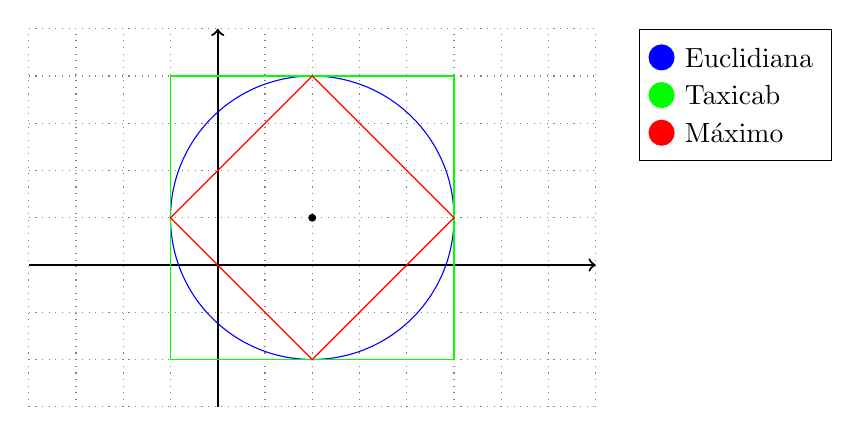
\begin{tikzpicture}[scale=0.6]
            \draw[gray, dotted] (0, 0) grid (12, 8);

            \draw[thick, ->] (0, 3) -- (12, 3);
            \draw[thick, ->] (4, 0) -- (4, 8);

            \draw[fill] (6, 4) circle (2pt);
            \draw[blue] (6, 4) circle (3);
            \draw[green] (3, 1) rectangle (9, 7);
            \draw[red] (6, 1) -- (9, 4) -- (6, 7) -- (3, 4) -- (6, 1);

            \matrix [draw,below left] at (17, 8) {
              \node [shape=circle, fill=blue, label=right:Euclidiana] {}; \\
              \node [shape=circle, fill=green, label=right:Taxicab] {}; \\
              \node [shape=circle, fill=red, label=right:Máximo] {}; \\
            };

        \end{tikzpicture}
    \end{center}
\end{frame}

\begin{frame}[fragile]{Representação de círculos}

    \begin{itemize}
        \item Um círculo pode ser representado através do ponto $C$ e do raio $r$

        \item A equação do círculo pode ser deduzida a partir da expressão $d(P, C) = r$, onde 
            $P = (x, y)$ é um ponto do círculo, $C = (x_0, y_0)$ é o centro do círculo e 
            $r$ é o raio

        \item A equação geral do círculo é dada por
        \[
            (x - x_0)^2 + (y - y_0)^2 = r^2
        \]

        \item Esta equação é útil para resolver vários problemas envolvendo círculos, como o 
            problema de determinar se um ponto está dentro, fora ou sobre um círculo
    \end{itemize}

        \inputcode{cpp}{circle.cpp}

\end{frame}

